\section{Victory Points}

\noindent
Bei \textit{Team-}Turnieren wird die Differenz der \imps einer Runde zwischen je
zwei Teams berechnet. Abhängig von der Anzahl der in diesem Durchgang gespielten \bos
wird die Differenz der \imps anschließend in \vps umgerechnet.\\[.1cm]
Die Anzahl der \vps zweier, sich gegenüber stehender, \textit{Teams} muss sich
auf exakt $20$ aufsummieren lassen.

\begin{center}
  \begin{tabular}{|l|}
    \hline
    \multicolumn{1}{|c|}{\ccb \textbf{Fachliteratur - Victory Points}}\\
    \hline
    \multicolumn{1}{|c|}{\cca \textbf{Literatur/Link}}\\
    \hline\hline
    \href{http://www.worldbridge.org/wp-content/uploads/2016/12/WBFVPscales.pdf}{World Bridge Federation}\\
    \hline
  \end{tabular}
\end{center}

\noindent
Die genaue Skalierung der Umrechnung in \textit{Victory Points} wird von der \text{World Bridge Federation} festgelegt und kann im folgenden Unterkapitel eingesehen werden.

\newpage

\subsection{WBF Continuozs VP Scale}
\noindent
\begin{figure}[ht]
	\centering
  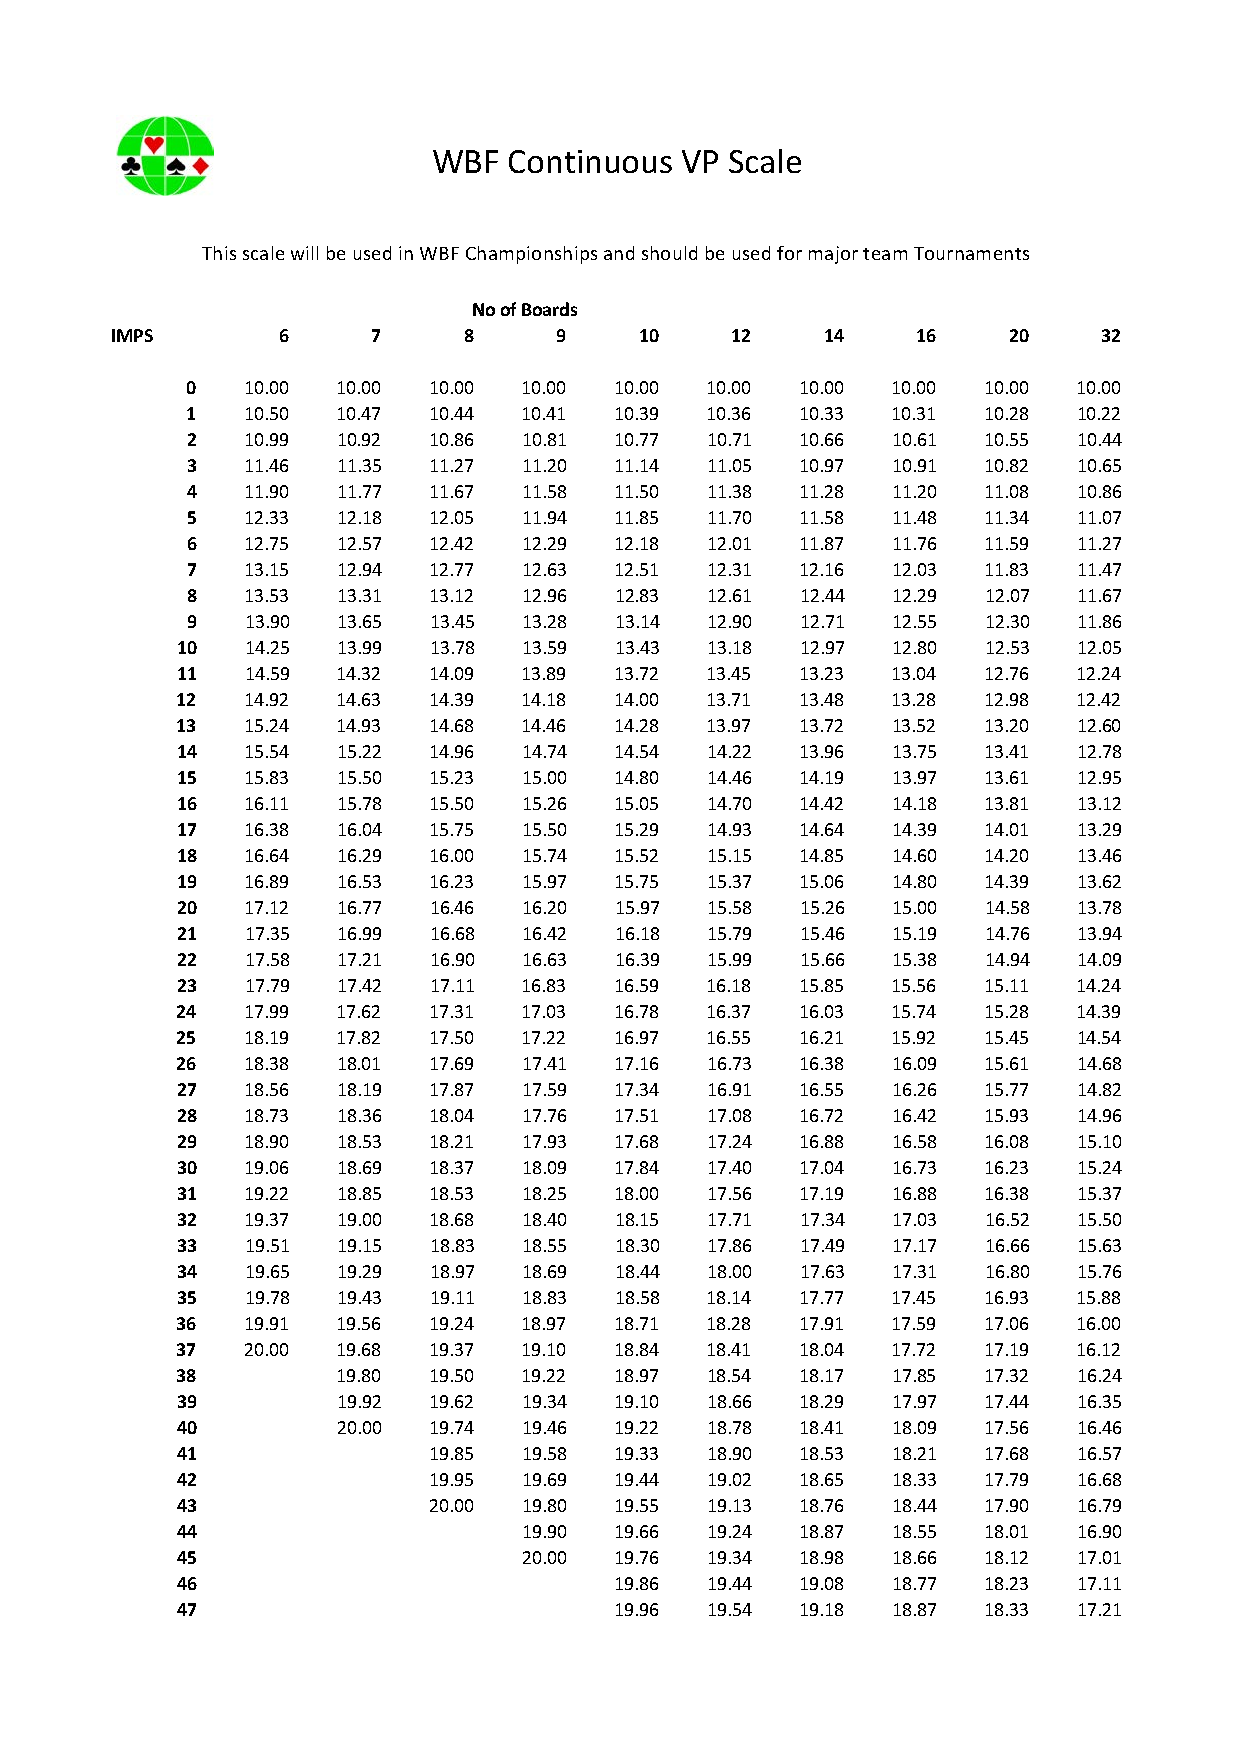
\includepdf[pages=1,pagecommand={},width=\textwidth]{references/WBFVPscales.pdf}
	\label{pdf/WBFVPscales}
\end{figure}
\newpage

\noindent
\begin{figure}[ht]
	\centering
  \includepdf[pages=2,pagecommand={},width=\textwidth]{references/WBFVPscales.pdf}
	\label{pdf/WBFVPscales}
\end{figure}
